\documentclass[10pt,a4paper]{report}
\usepackage[utf8]{inputenc}
\usepackage[francais]{babel}
\usepackage[T1]{fontenc}
\usepackage{amsmath}
\usepackage{amsfonts}
\usepackage{amssymb}
\usepackage{listings} % code highlights
\usepackage{fancyhdr} % headers and footers
\usepackage{graphicx}
\usepackage[left=2cm,right=2cm,top=2cm,bottom=2cm]{geometry}
\usepackage[nottoc]{tocbibind}


\author{Anuta Christian,Givron Azim}
\title{The frisbee's aerodynamism}


% Hide chapters numbers 
\renewcommand{\thesection}{\arabic{section}}


% Set headers and footers
\pagestyle{fancy}
\fancyhf{}
\lfoot{MECA-H3001: fluid mechanics and transfer process}
\cfoot{\thepage}
\renewcommand{\headrulewidth}{0pt}   % head horizontal rule 
\renewcommand{\footrulewidth}{0.5pt} % foot horizontal rule



\begin{document}



\begin{titlepage}


\includegraphics[scale=0.5]{logo-polytech-ULB-FR.jpg}

\center 
\vspace{5cm}
\textsc{\large MECA-H3001} \\[0.5cm]
\textsc{\LARGE Fluid mechanics and transfer process} \\[1.5cm]
\textsc{\Large English report} %\\[1.5cm]

\rule{\textwidth}{1pt}

\vspace{2cm}

\textsc{\large Anuta Christian, Givron Azim}

\end{titlepage}



\tableofcontents
\newpage 
\listoffigures
\newpage
\section{Introduction}
The frisbee is one of the objects that was invented decades ago and which is still used today. It is a source of amusement for kids and grown-ups. It also leads to the creation of new sports such as the ultimate frisbee or the disc golf. The particular shape of the frisbee allows it to glide for really long distances but to make the most of it, the toss has to be well oriented. In order to find the optimal angle, we need to first understand how it can fly. It can be easily explain with two simple considerations. On one hand we know that the aire has to flow around the frisbee, and the frisbee's shape forces the aire traveling above it to travel faster than the one below, while on the other hand, bernoulli's equation state that the pressure is low at locations where the flow velocity is high and vice-versa. This allows us to conclude that the pressure exerts under the frisbee is higher than the one exerts above it, that is what make it fly. The difference of pressure between both sides of the frisbee is due to a force pointing upward, normal to the flow direction, it is called the lift. 

\section{Method}
In order to find the optimal throw, we simulated the frisbee's trajectory by computing simulation. This requiere to know the velocity and the position of the frisbee at anytime. Since the acceleration modify the velocity through time, we should thus calculate it. This is possible by using the second law of Newton $F = ma$ where $F$ is a force and $m$ and $a$ are respectively the mass and the acceleration of the system. We finally see that the trajectory is indirectly given by the forces acting on the frisbee. The main ones are the gravitational force and the lift and drag forces. The latter is the force exerts by the air on the frisbee in the flow direction, it is the air resistance. Since these force only acte in the directions parallel and perpendicular to the flow, the simulation can be simplified by only considering those two dimensions.

\begin{figure}[h]
\centering
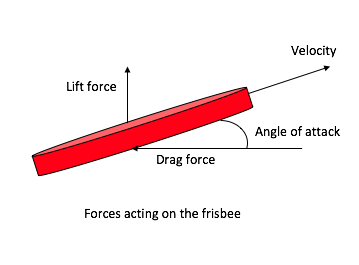
\includegraphics[scale=0.8]{forces.jpg}
\caption{Forces acting on the frisbee}
\label{Forces acting on the frisbee}
\end{figure}

\subsection{Mathematical decription}
The three forces cited above are all expressed by physical relationships. In the following part, we will present these relationships.The gravitational force $F_g$ exert on the frisbee is directly proportional to its mass $m$
\[F_g = m g\]
with $g$, the gravitational acceleration.
\\
The resolution of the equations to obtain the drag and lifts forces can be very difficult to solve because they depend on the geometry of the object studied. Fortunately, we can approximate the frisbee's geometry to a flat plate moving alongside the flow. In this case, the drag and lift forces are respectively given by :
\[F_d = -\frac{C_d \rho A  v^2}{2}\]
\[F_l = \frac{C_l \rho A  v^2}{2}\]
In this particular case, the fluid is the air, thus $\rho$ is its density, $v$ is the velocity of the Frisbee relative to the air, A is the surface area of the plate exposed to the air flow and $C_d$ and $C_l$ are respectively the drag and lift coefficients.
The drag coefficient, in general, depends on the Reynolds number which gives the type of flow studying. A flow can be laminar or turbulent. The first one concerns ordered flows while the second one caracterize chaotics flows. This number can be calculated with the following relationship:
\[\Re = \frac{\rho v d}{\eta}\]
where the only new term appearing here is $\eta$, the viscosity of the air.
By using the data presented at the result section, we found $Re=2.59$ $10^5$ which correspond to a turbulent flow.
This leads us to another equation:
\[C_d = C_{d0} + C_{d\alpha}(\alpha-\alpha_0)^2\]
which links the drag coefficient $C_d$ to the angle of attack $\alpha$ and the other terms $C_{d0}$, $C_{d\alpha}$ and $\alpha_0$ are constants, found experimentally.
\\Finally, the lift coefficient can be found with the relationship below:
\[C_l = C_{l0} + C_{l \alpha} \alpha\]
where $C_{l0}$ and $C_{l\alpha}$ are also constant found experimentally.
\subsection{Numerical modelling}
Solving this problem numerically can be done by using different methods. Here, we will use the Euler progressive method. It simply means that position is calculated from the previous one.
The initial conditions are given by :
\[x = 0 m\]
\[y = 1 m\]
\[v_x = v_i cos\alpha \]
\[v_y = v_i sin\alpha \] 
\begin{figure}[!h]
\centering
\includegraphics[scale=0.7]{initial.jpg}
\caption{Initial conditions}
\label{Initial conditions}
\end{figure}
where x is the horizontal position, y is the vertical one and $v_x$ and $v_y$ are respectively the horizontal and vertical velocity.
The next positions are calculated by :
\[x_{next} = x_{previous} + v_{x_{previous}} \Delta t \]
\[a_x=\frac{v_{x_{next}}}{\Delta t} = -\frac{C_d \rho A  v_{x_{previous}}^2}{2m}\]
\[y_{next} = y_{previous} + v_{y_{previous}} \Delta t \]
\[a_y = \frac{v_{y_{next}}}{\Delta t} = \frac{C_l \rho A  v_{y_{previous}}^2}{2m} - g\]
where $\Delta t$ is the time spent between two successive positions
\section{Results}
In this section, we will present three graphs that we obtain from the simulation. All of them were made with the same parameters values except for the angle of attack which is varying from $5\,^{\circ}$ up to $45\,^{\circ} $. 
\\The parameters values are the following:
TO DO ADD BOARD WITH THE CONSTANTS
\begin{figure}[!h]
 \centering
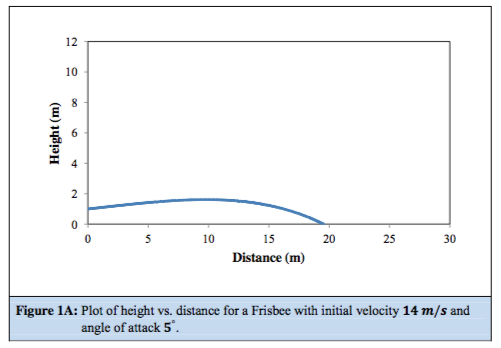
\includegraphics[scale=0.6]{graph1.jpg}
\caption{First result}
\label{First result}
\end{figure}
\\The first graph shows that an angle of attack of $5\,^{\circ}$ permit to the frisbee to reach a distance of $19m$.
\begin{figure}[!h]
\centering
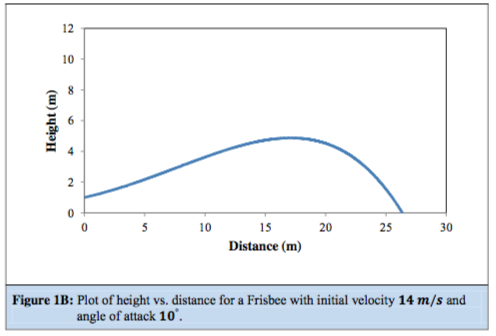
\includegraphics[scale=0.6]{graph2.jpg}
\caption{Second result}
\label{Second result}
\end{figure}
\\The second one, thrown with an angle of $10\,^{\circ}$ travelled for $26m$.
\begin{figure}[!h]
\centering
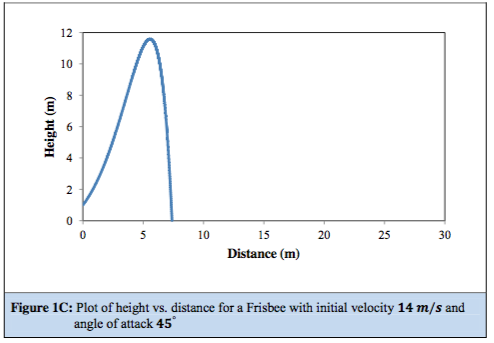
\includegraphics[scale=0.6]{graph3.jpg}
\caption{Third result}
\label{Third result}
\end{figure}
\\The last one only glide for $8m$ but was tossed with an angle of $45\,^{\circ} $.

\section{Discussion}
We saw in the different graphs that the angle of attack has an important impact on the distance travelled by the frisbee. It seems like the optimal angle is about $10\,^{\circ}$ since it gave the best results. At first, we would rather think that a $45\,^{\circ}$ inclination will allow a higher lift, since it is the vertical projection of the force applied on the frisbee by the flow, as shown on the scheme below.
\begin{figure}[!h]
\centering
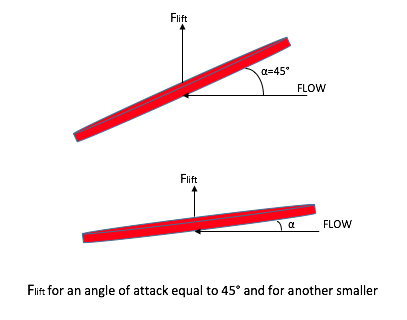
\includegraphics[scale=0.6]{intuitive.jpg}
\caption{Lift cause by the flow for different angle}
\label{Lift cause by the flow for different angle}
\end{figure}
In reality, it is not the case and it is explainable by introducing the concept of recirculation region. When the frisbee's inclination is not null, there is a flow separation. This create two different areas at different pressure. The pressure's difference forces the flow to come back in the region where the pressure is lower which is behind the frisbee, and is called the recirculation region. This movement of air is opposed to the flow direction, thus it increases the drag force which slow down the frisbee. An angle shorter than $10\,^{\circ}$ is neither optimal because the lift will than be to low.
\section{Conclusion}

\begin{thebibliography}{9}

\bibitem{art1}
  Hummel, Sarah A.,
  “Frisbee Flight Simulation and Throw Biomechanics”,
  University of Missouri,
  2003.
  
 \bibitem{art2}
  Lissaman P., Hubbard M.,
  “Maximum range of flying discs”,
  University of California,
  2010.
  
  \bibitem{art3}
  Morrison V. R.,
  “The Physics of Frisbees”,
  Mount Allison University,
  2005.

\bibitem{art4}
  Koyanagi R., Seob K., Ohta K., Ohgi Y.,
  “A computer simulation of the flying disc based on the wind tunnel test data”,
  University of Keio \& Yamagata,
  2012.
  
  \bibitem{art5}
  Baumback, Kathleen,
  “The Aerodynamics of Frisbee Flight”,
  University of South Florida,
  2010.
  
  \bibitem{art6}
  Erynn J. Schroeder,
  “An Aerodynamic Simulation of Disc Flight”,
  College of Saint Benedict/Saint John's University,
  2015.

\end{thebibliography}
\end{document}